
\begin{minipage}[t]{0.45\textwidth}
    \exo{Raisonner}{CentreSymAx1}
    
    \begin{figure}[H]
        \centering
        \begin{tikzpicture}[scale=0.8]
            \def\mypath{(-2,-2) -- (-1,1) --(-2,0) -- (-1,1.5)--(0,0)--(-2,-2)}
            \draw [white](-3,-3) grid (4,4);
            \draw [thick]\mypath ;
            \draw (0,-2)--(0,3) node [right]{$(d)$} ;
            \draw [dashed,cm={-1,0,0,1,(0,0)}] \mypath;%Matrice de transformation inverse X et Y 
        \end{tikzpicture}
    \end{figure}
\end{minipage}
\hfill
\begin{minipage}[t]{0.45\textwidth}
    \exo{Raisonner}{CentreSymAx2}
    
    \begin{figure}[H]
        \centering
        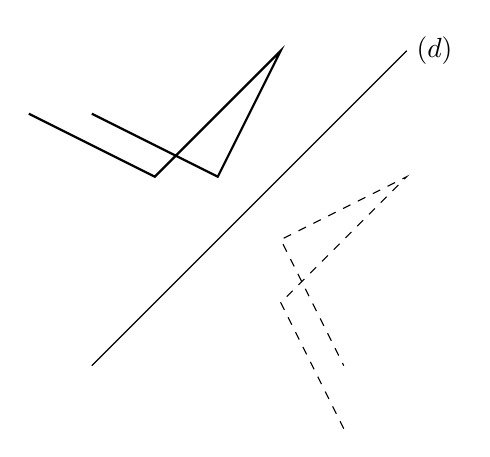
\begin{tikzpicture}[scale=0.8]
            \def\mypath{(-3,2) -- (-1,1) --(0,2) -- (1,3)--(0,1)--(-2,2)}
            \draw [thick]\mypath ;
            \draw (-2,-2)--(3,3) node [right]{$(d)$} ;
            \draw [dashed,cm={0,1,1,0,(0,0)}] \mypath;%Matrice de transformation inverse X et Y
        \end{tikzpicture}
    \end{figure}
\end{minipage}

\vspace*{-1em}


\begin{minipage}[t]{0.45\textwidth}
    \exo{Raisonner}{CentreSymAx3}
    
    \begin{figure}[H]
        \centering
        \begin{tikzpicture}[scale=0.8]
            \def\mypath{(1,-2) -- (0,-1) --(3,-2) -- (2,-1)--(-1,-1)--(1,-2)}
            \draw [white](-3,-3) grid (4,4);
            \draw [thick]\mypath ;
            \draw (-2,0)--(3,0) node [right]{$(d)$} ;
            \draw [dashed,cm={0,1,1,0,(0,0)}] \mypath;%Matrice de transformation inverse X et Y
        \end{tikzpicture}
    \end{figure}
\end{minipage}
\hfill
\begin{minipage}[t]{0.45\textwidth}
    \exo{Raisonner}{CentreSymAx4}
    
    \begin{figure}[H]
        \centering
        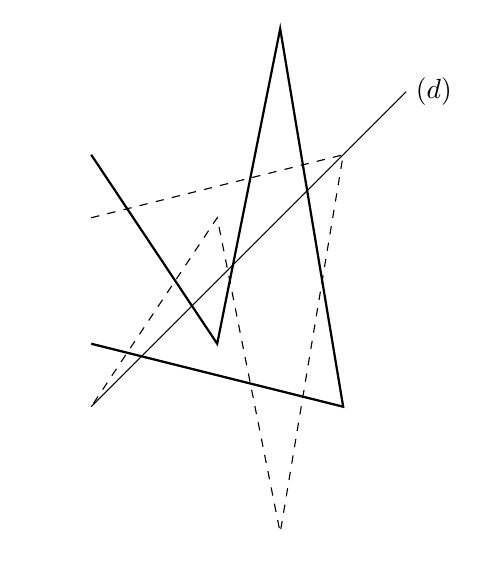
\begin{tikzpicture}[scale=0.8]
            \def\mypath{(-2,-1) -- (2,-2) --(1,4) -- (0,-1)--(-2,2)}
            \draw [white](-3,-3) grid (4,4);
            \draw [thick]\mypath ;
            \draw (-2,-2)--(3,3) node [right]{$(d)$} ;
            \draw [dashed,cm={1,0,0,-1,(0,0)}] \mypath;%Matrice de transformation inverse X et Y
        \end{tikzpicture}
    \end{figure}
\end{minipage}

\vspace*{-1em}


\begin{minipage}[t]{0.45\textwidth}
    \exo{Représenter}{CentreSymCent1}
    
    \begin{figure}[H]
        \centering
        \begin{tikzpicture}[scale=0.8]
            \tikzset{
                homothety at/.style args={#1 scaled by #2}{shift={($(#1)!#2!(0,0)$)},scale=#2},}
            \def\mypath{(-2,-2) -- (-1,1) --(-2,0) -- (-1,1.5)--(0,0)--(-2,-2)}
            \draw [white](-3,-3) grid (4,4);
            \fill[black] (0,0) coordinate (c) circle(2pt) node [above] {$O$};
            \draw [thick]\mypath ;
            \begin{scope}[homothety at=c scaled by -1]
                \draw [dashed]\mypath;
            \end{scope}
        \end{tikzpicture}
    \end{figure}
\end{minipage}
\hfill
\begin{minipage}[t]{0.45\textwidth}
    \exo{Représenter}{CentreSymCent2}
    
    \begin{figure}[H]
        \centering
        \begin{tikzpicture}[scale=0.8]
            \tikzset{
                homothety at/.style args={#1 scaled by #2}{shift={($(#1)!#2!(0,0)$)},scale=#2},}
            \def\mypath{(-3,2) -- (-1,1) --(0,2) -- (1,3)--(0,1)--(-2,2)}
            \fill[black] (1,0) coordinate (c) circle(2pt) node [above] {$O$};
            \draw [white](-3,-3) grid (4,4);
            \draw [thick]\mypath ;
            \begin{scope}[homothety at=c scaled by -1]
                \draw[dashed] \mypath;
            \end{scope}
        \end{tikzpicture}
    \end{figure}
\end{minipage}


\begin{minipage}[t]{0.45\textwidth}
    \exo{Représenter}{CentreSymCent3}
    
    \begin{figure}[H]
        \centering
        \begin{tikzpicture}[scale=0.8]
            \tikzset{
                homothety at/.style args={#1 scaled by #2}{shift={($(#1)!#2!(0,0)$)},scale=#2},}
            \def\mypath{(1,-2) -- (0,-1) --(3,-2) -- (2,-1)--(-1,-1)--(1,-2)}
            \fill [black](0,0) coordinate (c) circle(2pt) node [above] {$O$};
            \draw [white](-3,-3) grid (4,4);
            \draw [thick]\mypath ;
            \begin{scope}[homothety at=c scaled by -1]
                \draw [dashed]\mypath;
            \end{scope}
        \end{tikzpicture}
    \end{figure}
\end{minipage}
\hfill
\begin{minipage}[t]{0.45\textwidth}
    \exo{Représenter}{CentreSymCent4}
    
    \begin{figure}[H]
        \centering
        \begin{tikzpicture}[scale=0.8]
            \tikzset{
                homothety at/.style args={#1 scaled by #2}{shift={($(#1)!#2!(0,0)$)},scale=#2},}
            \def\mypath{(-2,-1) -- (2,-2) --(1,4) -- (0,-1)--(-2,2)}
            \fill [black](0,1) coordinate (c) circle(2pt) node [above] {$O$};
            \draw [white](-3,-3) grid (4,4);
            \draw [thick]\mypath ;
            \begin{scope}[homothety at=c scaled by -1]
                \draw [dashed]\mypath;
            \end{scope}
        \end{tikzpicture}
    \end{figure}
\end{minipage}


\begin{minipage}[t]{0.45\textwidth}
    \exo{Représenter}{CentreSymCent5}
    
    \begin{figure}[H]
        \centering
        \begin{tikzpicture}[scale=0.8]
            \tikzset{
                homothety at/.style args={#1 scaled by #2}{shift={($(#1)!#2!(0,0)$)},scale=#2},}
            \def\mypath{(1,-2) -- (0,-1) --(3,-2) -- (2,-1)--(-1,-1)--(1,-2)}
            \fill [black](1,1) coordinate (c) circle(2pt) node [above] {$O$};
            \draw [white](-3,-3) grid (4,4);
            \draw [thick]\mypath ;
            \begin{scope}[homothety at=c scaled by -1]
                \draw [dashed]\mypath;
            \end{scope}
        \end{tikzpicture}
    \end{figure}
\end{minipage}
\hfill
\begin{minipage}[t]{0.45\textwidth}
    \exo{Représenter}{CentreSymCent6}
    
    \begin{figure}[H]
        \centering
        \begin{tikzpicture}[scale=0.8]
            \tikzset{
                homothety at/.style args={#1 scaled by #2}{shift={($(#1)!#2!(0,0)$)},scale=#2},}
            \def\mypath{(-2,-1) -- (2,-2) --(1,4) -- (0,-1)--(-2,2)}
            \fill [black](-1,-0.5) coordinate (c) circle(2pt) node [above] {$O$};
            \draw [white](-3,-3) grid (4,4);
            \draw [thick]\mypath ;
            \begin{scope}[homothety at=c scaled by -1]
                \draw [dashed]\mypath;
            \end{scope}
        \end{tikzpicture}
    \end{figure}
\end{minipage}


\begin{minipage}[t]{0.45\textwidth}
    \exo{Représenter}{CentreSymCent7}
    
    \begin{figure}[H]
        \centering
        \begin{tikzpicture}[scale=0.8]
            \tikzset{
                homothety at/.style args={#1 scaled by #2}{shift={($(#1)!#2!(0,0)$)},scale=#2},}
            \def\mypath{(-2,1) -- (0,-1) --(3,3) -- (2,-1)--(-1,-1)--(1,-2)}
            \fill [black](0,0) coordinate (c) circle(2pt) node [above] {$O$};
            \draw [white](-3,-3) grid (4,4);
            \draw [thick]\mypath ;
            \begin{scope}[homothety at=c scaled by -1]
                \draw [dashed]\mypath;
            \end{scope}
        \end{tikzpicture}
    \end{figure}
\end{minipage}
\hfill
\begin{minipage}[t]{0.45\textwidth}
    \exo{Représenter}{CentreSymCent8}
    
    \begin{figure}[H]
        \centering
        \begin{tikzpicture}[scale=0.8]
            \tikzset{
                homothety at/.style args={#1 scaled by #2}{shift={($(#1)!#2!(0,0)$)},scale=#2},}
            \def\mypath{(-2,1) -- (0,-1) --(3,3) -- (2,-1)--(-1,-1)--(1,-2)}
            \fill [black](1,1) coordinate (c) circle(2pt) node [above] {$O$};
            \draw [white](-3,-3) grid (4,4);
            \draw [thick]\mypath ;
            \begin{scope}[homothety at=c scaled by -1]
                \draw [dashed]\mypath;
            \end{scope}
        \end{tikzpicture}
    \end{figure}
\end{minipage}